% =============================================================================
%  BM4322 Genomic Signal Processing - Assignment 1
%  Promoter Discovery in Bacteria  (report)
%  Compile with pdfLaTeX (e.g. on Overleaf). Figures are in the figures/ folder.
% =============================================================================
\documentclass[11pt,a4paper]{article}

% ---- Fill in your details here ----------------------------------------------
\newcommand{\studentname}{}          % e.g. \newcommand{\studentname}{A.B. Perera}
\newcommand{\indexno}{220472T}
% -----------------------------------------------------------------------------

\usepackage[margin=2.0cm,top=2.2cm,bottom=2.2cm]{geometry}
\usepackage{amsmath,amssymb}
\usepackage{graphicx}
\usepackage{booktabs}
\usepackage{array}
\usepackage{float}
\usepackage[font=small,labelfont=bf]{caption}
\usepackage{xcolor}
\usepackage{tikz}
\usetikzlibrary{arrows.meta,decorations.pathreplacing}
\usepackage{listings}
\usepackage{enumitem}
\usepackage{fancyhdr}
\usepackage{microtype}
\usepackage[colorlinks=true,linkcolor=blue!50!black,citecolor=blue!50!black,urlcolor=blue!50!black]{hyperref}
\hypersetup{pdftitle={BM4322 Assignment 1: Promoter Discovery in Bacteria},pdfauthor={Index No. \indexno}}

\graphicspath{{figures/}}
% let LaTeX put more figures on a text page (fewer half-empty pages)
\renewcommand{\topfraction}{0.9}
\renewcommand{\bottomfraction}{0.8}
\renewcommand{\textfraction}{0.08}
\renewcommand{\floatpagefraction}{0.8}
\setcounter{topnumber}{3}
\setcounter{bottomnumber}{2}
\setcounter{totalnumber}{4}
\setlength{\parskip}{4pt}
\setlength{\parindent}{0pt}
\setlist{itemsep=2pt,topsep=3pt}
\renewcommand{\labelitemi}{$\bullet$}
\renewcommand{\labelitemii}{$\circ$}

\pagestyle{fancy}
\fancyhf{}
\lhead{\small BM4322 Genomic Signal Processing -- Assignment 1}
\rhead{\small \indexno}
\cfoot{\small \thepage}
\renewcommand{\headrulewidth}{0.4pt}

\lstset{language=Python, basicstyle=\ttfamily\footnotesize, keywordstyle=\color{blue!60!black},
  commentstyle=\color{green!40!black}, stringstyle=\color{red!50!black}, breaklines=true,
  frame=single, numbers=left, numberstyle=\tiny\color{gray}, columns=fullflexible}

\newcommand{\gene}[1]{\textit{#1}}
\newcommand{\seqs}[1]{\texttt{#1}}

\begin{document}

% ----------------------------------------------------------------- title block
\begin{center}
  {\large BM4322 Genomic Signal Processing}\\[4pt]
  {\LARGE\bfseries Assignment 1: Promoter Discovery in Bacteria}\\[8pt]
  \textit{Salmonella enterica} subsp.\ \textit{enterica} strain PartC-Senterica-RM8376
  \quad(accession ASM2286996v1)\\[6pt]
  \if\relax\detokenize\expandafter{\studentname}\relax\else\studentname\quad$\bullet$\quad\fi
  Index No.\ \indexno\quad$\bullet$\quad 2 October 2026
\end{center}
\vspace{4pt}\hrule\vspace{8pt}

% =============================================================================
\section{Introduction}
% =============================================================================
A promoter is the short region of DNA in front of a gene where RNA polymerase binds and starts to
make mRNA. In bacteria most genes are read by RNA polymerase together with the sigma factor
$\sigma^{70}$, which recognises two short boxes: the $-35$ box (consensus \seqs{TTGACA}) and the
$-10$ box or Pribnow box (consensus \seqs{TATAAT})~\cite{pribnow,harley}. The boxes sit about 35 and
10 bases before the transcription start site (TSS) and are about 17 bases apart. The $-10$ box is
where the two DNA strands are pulled apart, so it is rich in A and T (an A--T pair is held by two
hydrogen bonds while a G--C pair has three). In the IUPAC code the letter W (``weak'') means A or T,
so \seqs{TATAAT} can be written as \seqs{WWWWWW}. In this assignment the promoter is modelled in an
even simpler way, as the query \seqs{WWWW}.

From a signal processing point of view a genome is a very long discrete signal that can take only
four values (A, C, G and T), and finding a promoter is like detecting a short known pattern inside a
long noisy signal~\cite{anastassiou}. I used the two detectors from the module: a standard local
search (exact pattern matching with the Smith--Waterman algorithm) and a statistical alignment with a
position probability matrix (PPM), which works like a matched filter. My aims were to
\begin{enumerate}
  \item cut 100 bases upstream and 3 bases downstream of 1000 sense-strand genes and check the
        extraction using the start codon (Methionine),
  \item find \seqs{WWWW} with the local search (Q1) and count the consecutive Ws (Q2),
  \item build a PPM from the hits (Q3) and use it for a statistical alignment (Q4), and
  \item compare the two searches (Q5).
\end{enumerate}
Figure~\ref{fig:layout} shows the part of the DNA that I worked with for every gene.

\begin{figure}[htbp]
\centering
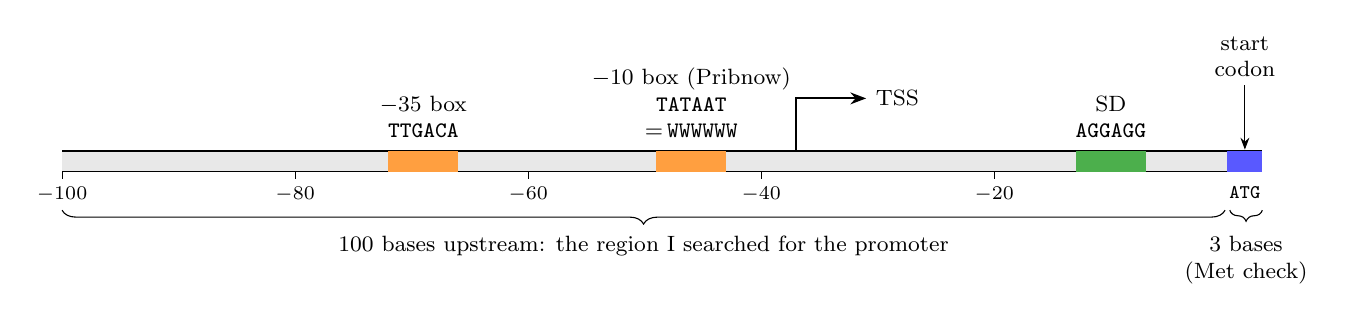
\begin{tikzpicture}[x=0.148cm,y=1cm,font=\footnotesize]
  % DNA double strand: x = position + 100 for upstream bases, start codon at x = 100..103
  \fill[gray!18] (0,-0.13) rectangle (103,0.13);
  \draw[semithick] (0,0.13) -- (103,0.13);
  \draw[semithick] (0,-0.13) -- (103,-0.13);
  % typical positions of the elements (they vary from gene to gene)
  \fill[orange!75] (28,-0.13) rectangle (34,0.13);        % -35 box, -72 to -67
  \fill[orange!75] (51,-0.13) rectangle (57,0.13);        % -10 box, -49 to -44
  \fill[green!55!black!70] (87,-0.13) rectangle (93,0.13); % SD, -13 to -8
  \fill[blue!65] (100,-0.13) rectangle (103,0.13);        % start codon
  \draw[thick,-{Stealth[length=2mm]}] (63,0.13) -- (63,0.8) -- (69,0.8);
  \node[above,align=center] at (31,0.18) {$-35$ box\\\seqs{TTGACA}};
  \node[above,align=center] at (54,0.18) {$-10$ box (Pribnow)\\\seqs{TATAAT}\\$=$\,\seqs{WWWWWW}};
  \node[right] at (69,0.8) {TSS};
  \node[above,align=center] at (90,0.18) {SD\\\seqs{AGGAGG}};
  \node[above,align=center] at (101.5,0.95) {start\\codon};
  \draw[{Stealth[length=1.5mm]}-] (101.5,0.15) -- (101.5,0.97);
  % position axis
  \foreach \p in {-100,-80,-60,-40,-20}{
    \draw (\p+100,-0.13) -- (\p+100,-0.22);
    \node[below,font=\scriptsize] at (\p+100,-0.2) {$\p$};
  }
  \node[below,font=\scriptsize] at (101.5,-0.2) {\seqs{ATG}};
  % braces
  \draw[decorate,decoration={brace,mirror,amplitude=5pt}] (0,-0.62) -- (99.8,-0.62)
     node[midway,below=6pt,align=center]{100 bases upstream: the region I searched for the promoter};
  \draw[decorate,decoration={brace,mirror,amplitude=4pt}] (100.2,-0.62) -- (103,-0.62)
     node[midway,below=6pt,align=center]{3 bases\\(Met check)};
\end{tikzpicture}
\caption{The 103-base sequence that I cut out for every gene. The two promoter boxes are about 17
bases apart. The positions of the $-35$ and $-10$ boxes, the transcription start site (TSS) and the
Shine--Dalgarno ribosome binding site (SD) are only typical; they change from gene to gene, and some
genes have no promoter of their own.}
\label{fig:layout}
\end{figure}

% =============================================================================
\section{Data used}
% =============================================================================
I downloaded the genome package of my accession (ASM2286996v1) from NCBI Datasets~\cite{ncbi}. The
package has many files, but I only needed the two shown in Table~\ref{tab:files}. All the analysis
was done in Python~3 (NumPy, pandas, Matplotlib and SciPy). I split the code into one file per
step of the assignment; \texttt{main.py} runs everything in one go, and a Jupyter notebook runs the
same functions step by step. Both are in the submitted \texttt{.zip} file (Appendix~A).

\begin{table}[htbp]
\centering
\caption{The data files I used and why.}
\label{tab:files}
\small
\begin{tabular}{>{\raggedright\arraybackslash}p{4.3cm}>{\raggedright\arraybackslash}p{5.4cm}>{\raggedright\arraybackslash}p{5.6cm}}
\toprule
File & What it contains & Why I used it\\
\midrule
\texttt{GCA\_022869965.1\_}\allowbreak\texttt{ASM2286996v1\_}\allowbreak\texttt{genomic.fna} (GenBank genome, FASTA) &
The DNA of the chromosome (4,857,492 bases) and of a 93,933-base plasmid, written as A, C, G and T. &
This is the ``signal'' that I searched. All 1000 sequences were cut out of it.\\[3pt]
\texttt{ncbi\_dataset.tsv} (protein table) &
One row per gene: chromosome, start (\texttt{Begin}), end (\texttt{End}), strand
(\texttt{Orientation}), gene type, protein length, locus tag and name. &
The genome itself has no labels, so this table tells me where each gene starts and on which
strand. I also used the protein length to check my code.\\
\bottomrule
\end{tabular}
\end{table}

The other files in the package were not needed. The GFF, GTF and GenBank flat files hold the same
gene annotation as the table in more complicated formats, and the CDS and protein FASTA files only
contain the genes themselves. The CDS file in particular cannot be used for this assignment because
it does not include the DNA in front of each gene, which is exactly where a promoter is.

One detail confused me at first: the table calls the chromosome \texttt{NZ\_CP064385.1} (its RefSeq
name) while the GenBank FASTA calls it \texttt{CP064385.1}. A RefSeq record is a copy of the GenBank
record, and I checked that the RefSeq and GenBank FASTA files in the package have exactly the same
sequence (same length and same MD5 checksum), so the positions in the table are valid for the GenBank
genome. The chromosome has 52.2\% G+C. The table lists 4,850 genes (4,612 protein-coding, 113
pseudogenes and 125 RNA genes); 4,733 of them are on the chromosome, 2,280 on the + strand and 2,453
on the $-$ strand. I only used the chromosome.

% =============================================================================
\section{Method and why I chose it}
% =============================================================================
\subsection{Choosing the genes and cutting the sequences}
The brief asks for genes of the sense strand, which I took to mean the genes on the + strand of the
chromosome (\texttt{Orientation = plus}). For these genes the DNA is read from left to right, so
``upstream'' simply means smaller positions and nothing has to be reverse-complemented. I kept only
protein-coding genes, because pseudogenes and RNA genes do not make a protein and therefore cannot be
checked with Methionine. One gene crosses the end of the circular chromosome (its \texttt{Begin} is
larger than its \texttt{End}), so I skipped it. From the remaining 2,153 genes I took the first 1000
in the order they appear on the chromosome, from \gene{murJ} (starting at base 571) to \gene{acpT}
(ending at base 2,496,884). I did not choose genes by hand, so the selection is not biased towards
genes with or without promoters.

The table uses 1-based positions (the first base of the genome is 1) but Python strings start at
index 0. For a gene whose first base is $b$, the start codon is at positions $b$ to $b+2$, so in
Python the 103-base sequence is \texttt{genome[b-101 : b+2]}, which covers positions $b-100$ to
$b+2$: 100 upstream bases followed by the start codon. I used 100 upstream bases because in
\textit{E.~coli}, a close relative of \textit{Salmonella}, the TSS is usually 20--40 bases in front of
the start codon~\cite{mendoza}, so the $-10$ and $-35$ boxes should normally fall inside this window
(Figure~\ref{fig:layout}). In this report I give positions relative to the start codon: the base just
before it is $-1$ and the farthest base is $-100$. The position of a hit is the position of its first
(5$'$) base, so a \seqs{WWWW} hit at $-90$ covers $-90$ to $-87$.

\subsection{Checking the extraction with Methionine}
An off-by-one mistake in the indexing would shift every sequence, so before anything else I checked
the 3 downstream bases. If the positions are right they must be a start codon, which codes for
Methionine. Table~\ref{tab:met} shows nine well-known genes: all of them have \seqs{ATG}, and their
translated proteins start with M and have exactly the length given in the table. Over all 1000 genes
the start codons were \seqs{ATG} (912), \seqs{GTG} (66), \seqs{TTG} (18), \seqs{ATT} (2) and \seqs{CTG}
(2). The non-ATG codons are normal in bacteria: at the start of a gene they are read by the initiator
tRNA that carries formyl-Methionine, so every protein still starts with Methionine. As a stronger
test I translated every whole coding sequence. 999 of the 1000 gave exactly the protein length in the
table and ended with a stop codon. The only exception was an IS3-family transposase
(IUJ38\_RS08235), which is known to need a ribosomal frameshift. This convinced me that my indexing
is correct.

\begin{table}[htbp]
\centering
\caption{Methionine check on known genes. Upstream bases in lower case, start codon in capitals.}
\label{tab:met}
\footnotesize
\setlength{\tabcolsep}{4pt}
\begin{tabular}{llllc}
\toprule
Gene & Locus tag & Last 12 bases + start codon & Start of my translation & Length (aa): table / mine\\
\midrule
\gene{murJ} & IUJ38\_RS00010 & \texttt{aatacaaaagaa ATG} & \texttt{MNLLKSLAAV\ldots} & 511 / 511\\
\gene{rpoD} & IUJ38\_RS10490 & \texttt{ggataccgtctt ATG} & \texttt{MEQNPQSQLK\ldots} & 615 / 615\\
\gene{crp}  & IUJ38\_RS11775 & \texttt{ggataaccgcgc ATG} & \texttt{MVLGKPQTDP\ldots} & 210 / 210\\
\gene{hns}  & IUJ38\_RS02980 & \texttt{gagattactaca ATG} & \texttt{MSEALKILNN\ldots} & 137 / 137\\
\gene{fis}  & IUJ38\_RS11365 & \texttt{gctgacagaact ATG} & \texttt{MFEQRVNSDV\ldots} & 98 / 98\\
\gene{ompC} & IUJ38\_RS01830 & \texttt{aaggcatataaa ATG} & \texttt{MKKVVVLSAV\ldots} & 372 / 372\\
\gene{hilA} & IUJ38\_RS08775 & \texttt{tacactattatc ATG} & \texttt{MPHFNPVPVS\ldots} & 553 / 553\\
\gene{tolC} & IUJ38\_RS10355 & \texttt{tcacaacaagga ATG} & \texttt{MQMKKLLPIL\ldots} & 491 / 491\\
\gene{trpA} & IUJ38\_RS02860 & \texttt{aggggaaatctg ATG} & \texttt{MERYENLFAQ\ldots} & 268 / 268\\
\bottomrule
\end{tabular}
\end{table}

\subsection{Q1: standard local search}
Because I am looking for a short query somewhere inside a longer sequence, I used local alignment
(the Smith--Waterman algorithm~\cite{sw}) and not global alignment, which would try to align the two
sequences from end to end. For the upstream sequence $x$ (100 bases) and the query $q=$~\seqs{WWWW},
the algorithm fills a score matrix
\begin{equation}
H(i,j)=\max\{\,0,\; H(i-1,j-1)+s(x_i,q_j),\; H(i-1,j)+g,\; H(i,j-1)+g\,\},
\label{eq:sw}
\end{equation}
where $s=+1$ when the base fits the query letter (A or T for W) and $s=-1$ otherwise, and the gap
penalty is $g=-2$. These are the same scores as in the local search code given in the module. The 0
in Equation~\eqref{eq:sw} lets an alignment start anywhere, which is what makes the search local, and
the best alignment is found by tracing back from the cell with the highest score.

The query is \emph{intact} when all of \seqs{WWWW} is aligned with no mismatch and no gap. With these
scores the highest possible score is 4 and only an intact match can reach it, so I counted a gene as
having a potential promoter when its best score was 4. When a sequence has several intact matches
they all score 4; like \texttt{max()} in MATLAB or NumPy, my code takes the first maximum, which is
the hit nearest the 5$'$ end (farthest from the gene). I searched only the 100 upstream bases,
because a promoter cannot overlap the start codon.

\subsection{Q2: consecutive Ws}
For every hit I counted how many A or T bases follow each other from the first base of the hit
towards the gene. A Pribnow box (\seqs{TATAAT}) would give 6, so this tells me whether the
\seqs{WWWW} is part of a longer A/T stretch. To judge the result I compared it with random DNA. If
every base is W with probability $p$, independently of the others, a run that already has 4 Ws
continues with probability $p$ at every step, so its length $L$ follows a geometric distribution
\begin{equation}
P(L=n)=p^{\,n-4}(1-p),\qquad n=4,5,6,\ldots
\label{eq:geo}
\end{equation}
I used $p=0.549$, the A/T fraction of my 1000 upstream regions (the whole genome has only 0.478).

\subsection{Q3: position probability matrix}
From each hit I took the 6 bases starting at the hit (whatever their C/G content, as the brief
says), because the Pribnow box is 6 bases long. I counted how many times each base $b$ appears at
each position $j$ (the position frequency matrix $n_{b,j}$) and turned the counts into probabilities
\begin{equation}
p_{b,j}=\frac{n_{b,j}+k}{N+4k},\qquad k=0.01,
\label{eq:ppm}
\end{equation}
where $N=995$ is the number of 6-base sequences. The small pseudocount $k$ is needed because some
bases never appear at some positions and $\ln 0$ would break the scores in Q4; 0.01 is the value used
in the module code. To see how much each position tells us, I calculated its information content
against a random base (probability 1/4 each),
\begin{equation}
I_j=\sum_{b\in\{A,C,G,T\}} p_{b,j}\log_2\frac{p_{b,j}}{0.25}\ \text{bits},
\label{eq:ic}
\end{equation}
which is 0 for a completely random position and 2 bits for a position that is always the same base,
and I drew a sequence logo~\cite{logo}.

\subsection{Q4: statistical alignment}
In the statistical alignment I slid a 6-base window along each upstream sequence (95 windows, from
$-100$ to $-6$) and scored every window with the log-likelihood of its bases under the PPM:
\begin{equation}
S(m)=\sum_{j=1}^{6}\ln p_{\,x_{m+j-1},\,j}.
\label{eq:score}
\end{equation}
This is like a matched filter: the PPM is the template, sliding it along the sequence is a
correlation, and the window with the largest output is the best alignment~\cite{stormo}. The highest
score any window can get is the score of the consensus (the most likely base at every position),
$S_{\text{cons}}=\sum_j \ln\max_b p_{b,j}$. I said that a promoter is present when
$S_{\text{best}}-S_{\text{cons}}\geq T$ and tried $T=-1,-2,-3,-4$ and $-5$, the same range used in
the module. For example, $T=-2$ means that the best window is at least $e^{-2}\approx 14\%$ as likely
as the consensus. For the comparison of positions in Q5 I used $T=-2$.

\subsection{Chance-level control}
A detector is only useful if it finds the pattern more often in real promoter regions than by chance.
To measure the chance level, I shuffled every upstream sequence 100 times (same bases, random order;
100,000 sequences in total) and ran both searches on the shuffled sequences. Shuffling keeps the A/T
content but destroys any real signal, so the shuffled result is what each detector reports when
there is nothing to find. For the shuffled sequences I used a regular expression instead of
Smith--Waterman to save time; on the real sequences the two gave exactly the same hits. To compare
the two position distributions in Q5 I used the two-sample Kolmogorov--Smirnov (KS) test.

% =============================================================================
\section{Results and discussion}
% =============================================================================
\subsection{Q1: local search for WWWW}
An intact \seqs{WWWW} was found in 995 of the 1000 upstream sequences, so \textbf{99.5\%} of the genes
have a potential promoter by this definition. The other five genes (\gene{holB}, IUJ38\_RS03200,
\gene{pduS}, \gene{srlE} and \gene{gltB}) only reached a score of 3. Their upstream regions are G+C
rich (61--66\% G+C), and for the first four the whole region lies inside the coding sequence of the
gene before them, which ends right on top of their start codon.

Figure~\ref{fig:q1} shows where the hits are. The distribution is strongly skewed to the far end of
the region: the median position is $-90$ (interquartile range $-97$ to $-77$), 135 hits are exactly
at $-100$ and 72.4\% of the hits are at $-80$ or further upstream.

\begin{figure}[htbp]
\centering
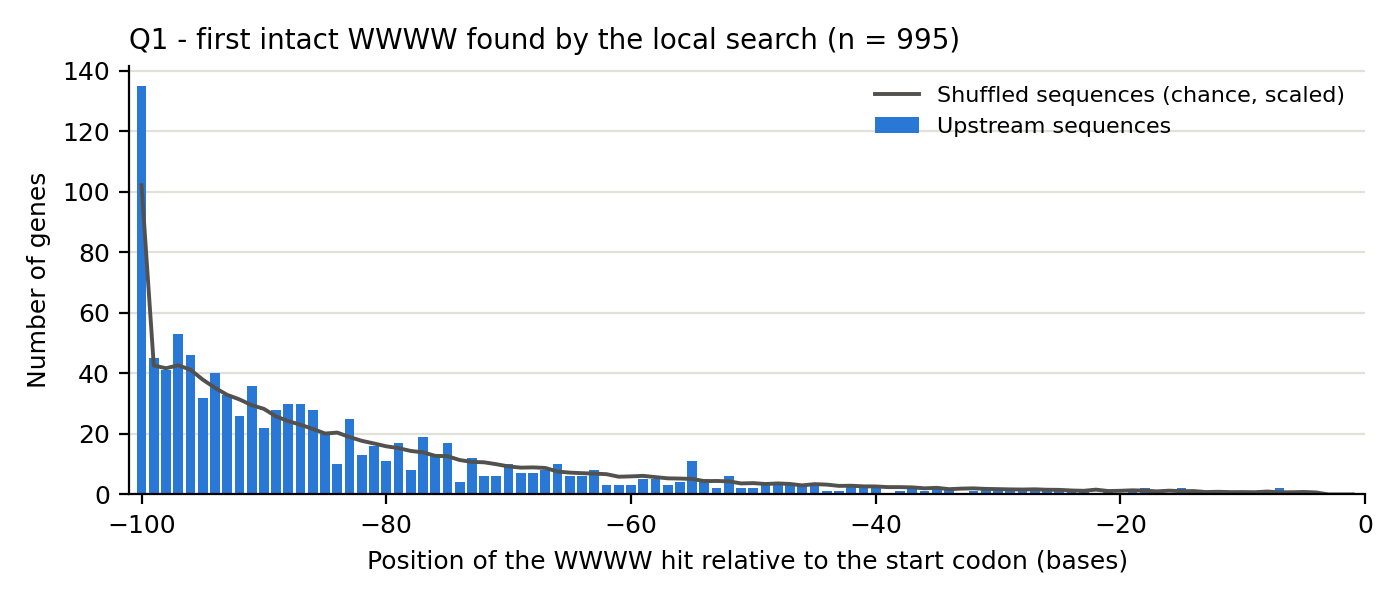
\includegraphics[width=0.86\linewidth]{fig_Q1_positions.png}
\caption{Q1: position of the first intact \seqs{WWWW} found by the local search (bars). The line is
the same distribution for the shuffled sequences, scaled to 995 genes.}
\label{fig:q1}
\end{figure}

At first this looked as if the promoters were far away from the genes, but it is really caused by
the way the search works. Each upstream sequence contains on average 12.2 intact \seqs{WWWW}
(median 11, range 0--42) and the local search reports only the first one it meets, starting from
$-100$. Figure~\ref{fig:q1} is therefore just the ``waiting time'' until the first A/T run, and the
shuffled sequences give almost the same curve (median $-88$). Figure~\ref{fig:occ} shows all 12,224
occurrences instead of only the first one. They are spread evenly, at about 12\% per position, up to
$-26$, rise to 15--17.5\% between $-25$ and $-15$, drop to 4--8\% for words starting between $-13$ and
$-9$, and rise again to about 16\% just before the start codon. The dip is the G-rich Shine--Dalgarno
(SD) ribosome binding site (consensus \seqs{AGGAGG})~\cite{sd}, which also shows up clearly as a drop
in A/T content in the lower panel. If I had taken the last hit (nearest the gene) instead of the
first, the median position would have been $-14$, which is also in this translation start region and
not at a $-10$ box.

\begin{figure}[htbp]
\centering
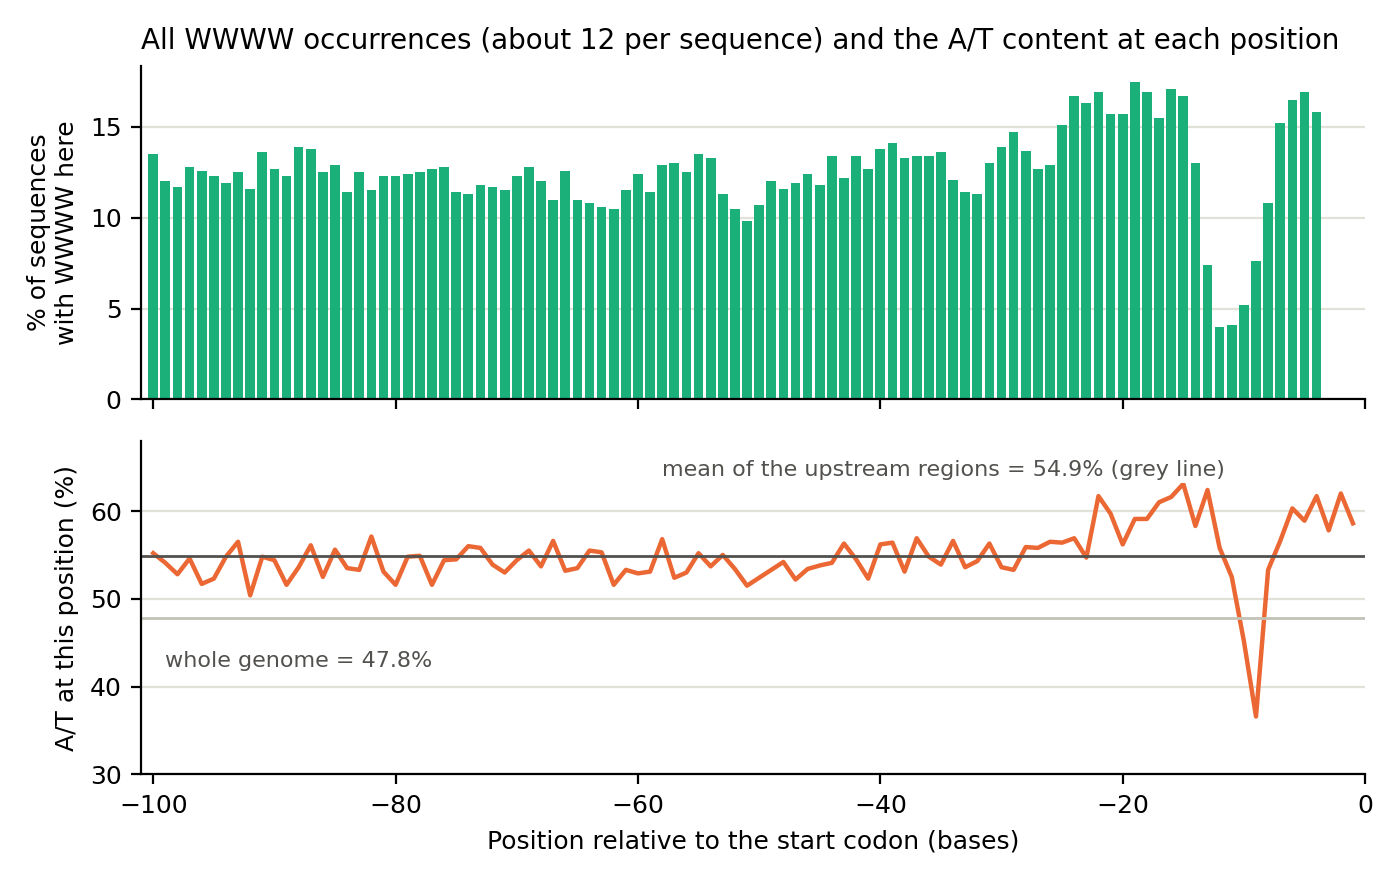
\includegraphics[width=0.8\linewidth]{fig_Q1_all_occurrences.png}
\caption{Top: percentage of the 1000 sequences with an intact \seqs{WWWW} starting at each position
(all occurrences, not only the first). Bottom: A/T content at each position. The dip at $-13$ to $-9$
is the Shine--Dalgarno site.}
\label{fig:occ}
\end{figure}

\subsection{Q2: number of consecutive Ws}
The A/T runs at the hits are 4 to 22 bases long, with a mean of 5.5 and a median of 5
(Table~\ref{tab:runs}, Figure~\ref{fig:q2}). Most runs are short, as expected for random DNA, but
compared with the geometric distribution of Equation~\eqref{eq:geo} there are fewer runs of exactly
four (381 against 449 expected) and more long runs (122 runs of 8 or more against 90). The longest
runs are 22 bases long, upstream of \gene{chbC} (\seqs{AATTAATTATTTTTTAATTTTT}) and \gene{ftnA}. The
real sequences also contain more \seqs{WWWW} words than their shuffled versions (12.2 against 9.7 per
sequence). So the upstream regions do contain real A/T tracts. Such tracts are common in bacterial
promoter regions because they make the DNA easier to open, but a long A/T run alone is not enough to
call a promoter.

\begin{table}[htbp]
\centering
\caption{Q2: number of consecutive Ws at the 995 hits, observed and expected for random DNA
(Equation~\ref{eq:geo}, $p=0.549$).}
\label{tab:runs}
\small
\setlength{\tabcolsep}{4.5pt}
\begin{tabular}{lrrrrrrrrrrrr}
\toprule
Consecutive Ws & 4 & 5 & 6 & 7 & 8 & 9 & 10 & 11 & 12 & 13 & 14 & $\geq 15$\\
\midrule
Genes (observed) & 381 & 247 & 157 & 88 & 53 & 33 & 16 & 6 & 4 & 6 & 2 & 2\\
Expected (random) & 448.6 & 246.3 & 135.3 & 74.3 & 40.8 & 22.4 & 12.3 & 6.8 & 3.7 & 2.0 & 1.1 & 1.4\\
\bottomrule
\end{tabular}
\end{table}

\begin{figure}[htbp]
\centering
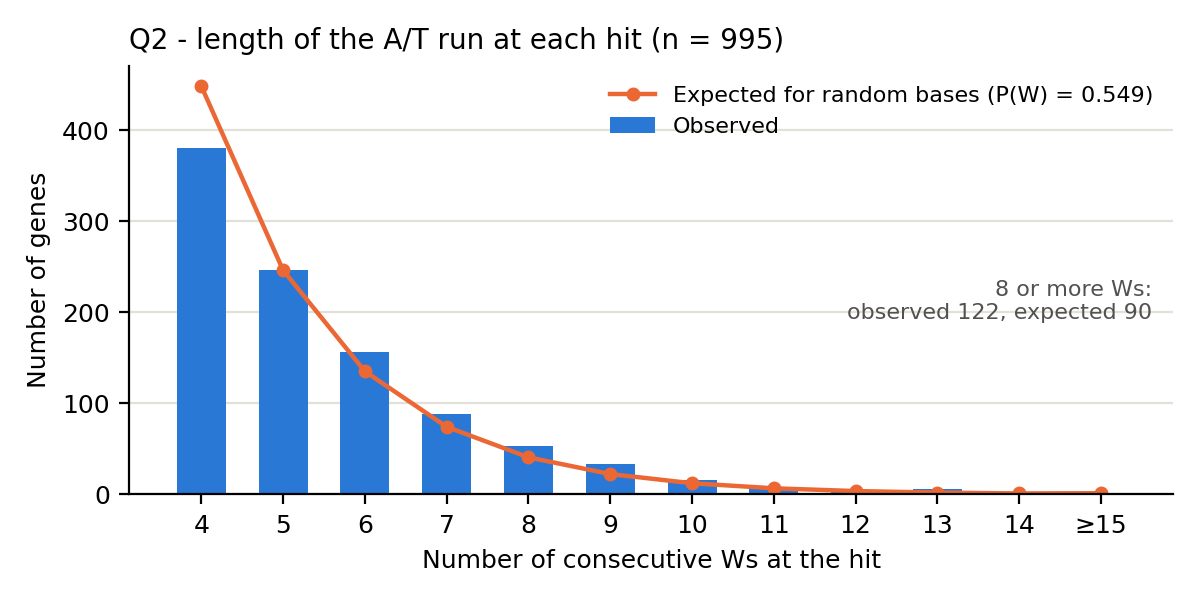
\includegraphics[width=0.66\linewidth]{fig_Q2_consecutive_W.png}
\caption{Q2: distribution of the number of consecutive Ws at each hit (bars) and the geometric
expectation for random DNA (line).}
\label{fig:q2}
\end{figure}

\subsection{Q3: position probability matrix}
The 995 six-base sequences (239 different ones; the most common were \seqs{AAAAAA} 18,
\seqs{TTTTTT} 15 and \seqs{TTTTTG} 15) gave the matrix in Table~\ref{tab:ppm} and the logo in
Figure~\ref{fig:q3}. Positions 1--4 contain only A and T, in almost equal amounts, because every
sequence starts with the \seqs{WWWW} found in Q1. Each of these positions carries about 1~bit, the
maximum for a choice between two letters. Positions 5 and 6 are close to random (0.05 and 0.01~bits;
A or T 62\% and 54\% of the time). The consensus is \seqs{ATTTTT} with a score of $-5.012$, and the
whole matrix holds only 4.06~bits. In other words, the PPM mostly gives back the query that I used to
find the hits. I also noticed that the W frequency at position 5 (0.617) is exactly the fraction of
hits whose run is longer than four bases (614/995), so the PPM and the Q2 distribution describe the
same A/T runs.

\begin{table}[htbp]
\centering
\caption{Q3: position probability matrix (counts in brackets) and information content. C and G at
positions 1--4 were never seen, so they only have the pseudocount ($p=1.0\times10^{-5}$).}
\label{tab:ppm}
\small
\begin{tabular}{lcccccc}
\toprule
Base & 1 & 2 & 3 & 4 & 5 & 6\\
\midrule
A & 0.520 (517) & 0.451 (449) & 0.485 (483) & 0.487 (485) & 0.294 (293) & 0.269 (268)\\
C & 0.000 (0) & 0.000 (0) & 0.000 (0) & 0.000 (0) & 0.221 (220) & 0.252 (251)\\
G & 0.000 (0) & 0.000 (0) & 0.000 (0) & 0.000 (0) & 0.162 (161) & 0.204 (203)\\
T & 0.480 (478) & 0.549 (546) & 0.515 (512) & 0.513 (510) & 0.323 (321) & 0.274 (273)\\
\midrule
Information (bits) & 1.00 & 1.01 & 1.00 & 1.00 & 0.05 & 0.01\\
\bottomrule
\end{tabular}
\end{table}

\begin{figure}[htbp]
\centering
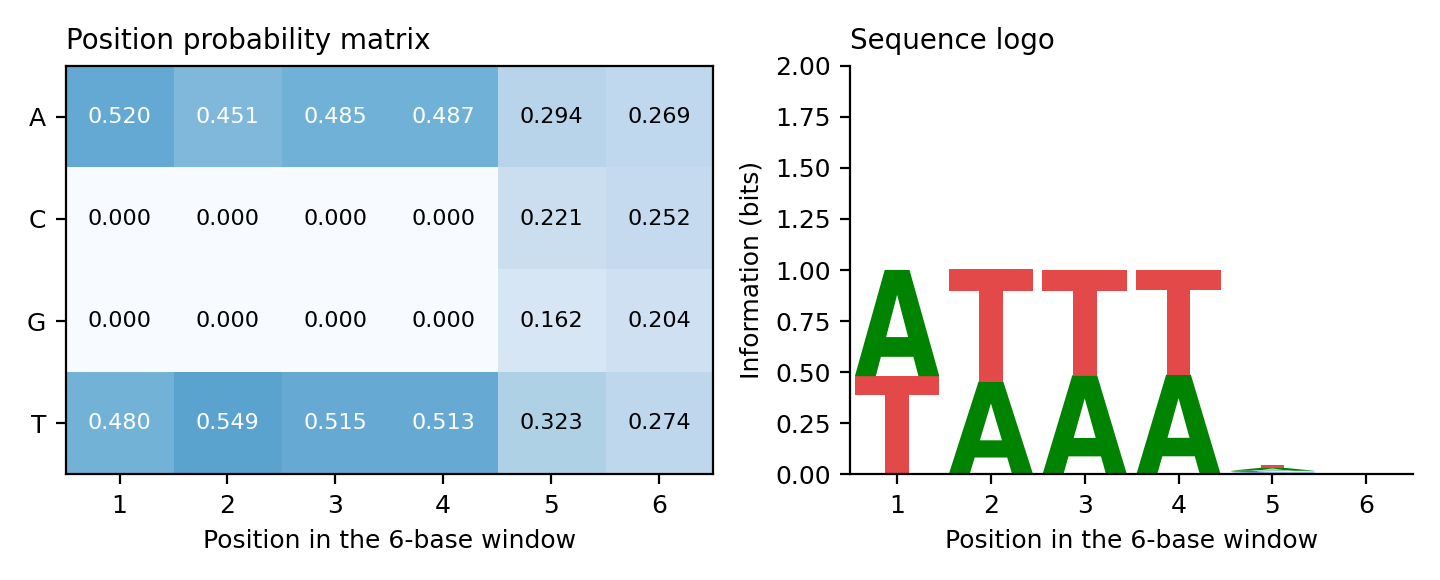
\includegraphics[width=0.82\linewidth]{fig_Q3_PPM_logo.png}
\caption{Q3: the PPM (left) and the sequence logo (right), where the height of each letter is its
probability times the information content of the position.}
\label{fig:q3}
\end{figure}

\subsection{Q4: statistical alignment}
Table~\ref{tab:thr} shows the percentage of genes whose best window passed each threshold. With
$T=-1$, 99.0\% of the genes were detected, and with $T=-2$ to $-5$, 99.5\%. Every window that passed
started with an intact \seqs{WWWW}. The reason is the pseudocount: a C or G at positions 1--4 has
$p\approx10^{-5}$, which costs about 10.9 (in ln units) compared with the consensus, much more than any
threshold I used. The five genes without \seqs{WWWW} had best scores 10.9 to 11.2 below the consensus
and were not detected. On the other hand, any window that starts with an intact \seqs{WWWW} scores
within 1.37 of the consensus, so every threshold of $-1.37$ or lower selects exactly the same genes as
the local search.

The best windows are spread over the whole region (median $-51$, interquartile range $-76$ to $-28$;
Figure~\ref{fig:q4}) and are mostly T-rich words close to the consensus: \seqs{ATTTTT} (113),
\seqs{ATTATT} (64), \seqs{ATTTTA} (56) and \seqs{TTTTTT} (43). 68.5\% of them contain only A and T.

\begin{table}[htbp]
\centering
\caption{Q4: percentage of genes detected by the statistical alignment for each threshold $T$
(best score minus consensus score), for my sequences and for the shuffled sequences.}
\label{tab:thr}
\small
\begin{tabular}{lccccc}
\toprule
Threshold $T$ & $-1$ & $-2$ & $-3$ & $-4$ & $-5$\\
\midrule
Upstream sequences & 99.0\% & 99.5\% & 99.5\% & 99.5\% & 99.5\%\\
Shuffled sequences & 96.2\% & 97.6\% & 97.6\% & 97.6\% & 97.6\%\\
\bottomrule
\end{tabular}
\end{table}

\begin{figure}[htbp]
\centering
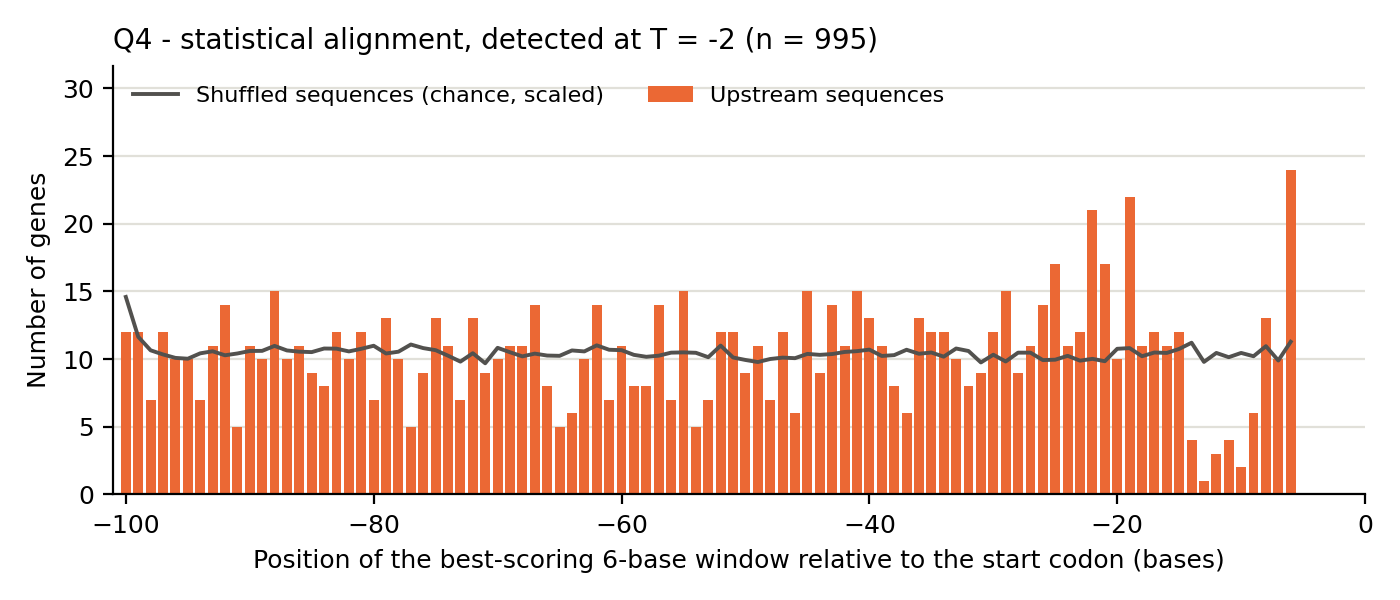
\includegraphics[width=0.86\linewidth]{fig_Q4_positions.png}
\caption{Q4: position of the best-scoring window for the 995 genes detected at $T=-2$ (bars) and the
same for the shuffled sequences (line, scaled).}
\label{fig:q4}
\end{figure}

\subsection{Q5: comparison of the two searches}
Table~\ref{tab:compare} puts the main numbers of the two searches side by side.

\begin{table}[htbp]
\centering
\caption{Q5: local search (Q1) against statistical alignment (Q4, $T=-2$).}
\label{tab:compare}
\small
\begin{tabular}{lcc}
\toprule
 & Local search & Statistical alignment\\
\midrule
Genes with a potential promoter & 995 (99.5\%) & 995 (99.5\%); 990 at $T=-1$\\
Same test on shuffled sequences & 97.8\% & 97.6\%\\
Position of the hit: median (IQR) & $-90$ ($-97$ to $-77$) & $-51$ ($-76$ to $-28$)\\
Mean A/T run length at the hit & 5.5 & 6.4\\
Same position in both searches & \multicolumn{2}{c}{179 genes (18.0\%); within 2 bases: 241 (24.2\%)}\\
KS test between the two positions & \multicolumn{2}{c}{$D=0.53$, $p<10^{-100}$}\\
\bottomrule
\end{tabular}
\end{table}

\begin{figure}[htbp]
\centering
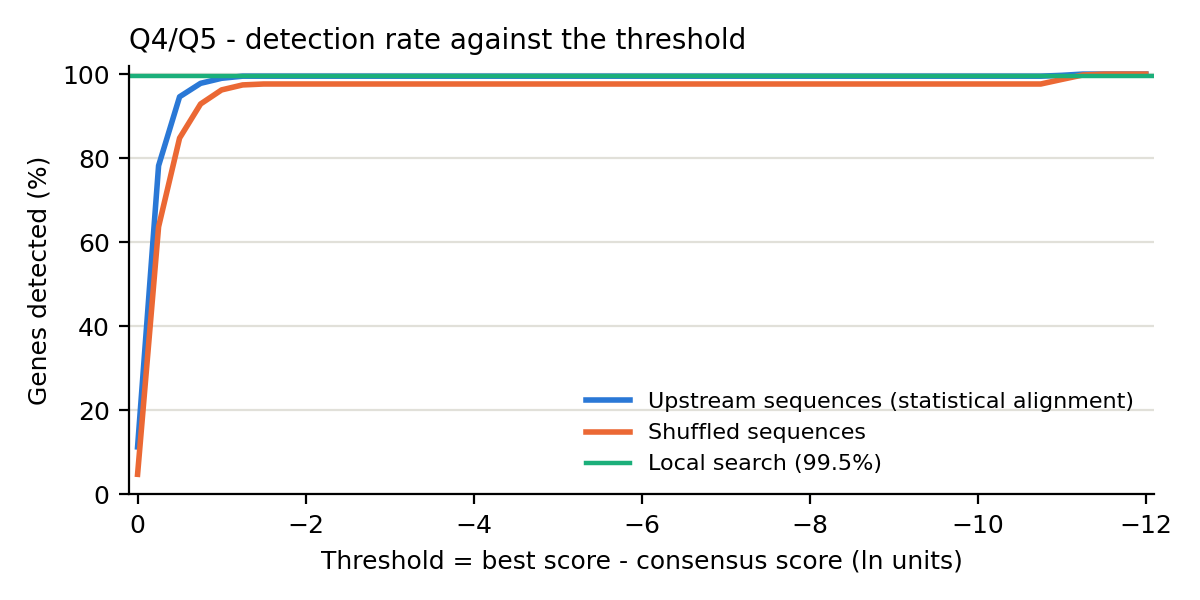
\includegraphics[width=0.64\linewidth]{fig_Q5_threshold.png}
\caption{Percentage of genes detected by the statistical alignment as the threshold changes, for my
sequences and for the shuffled sequences, compared with the local search.}
\label{fig:thr}
\end{figure}

\begin{figure}[htbp]
\centering
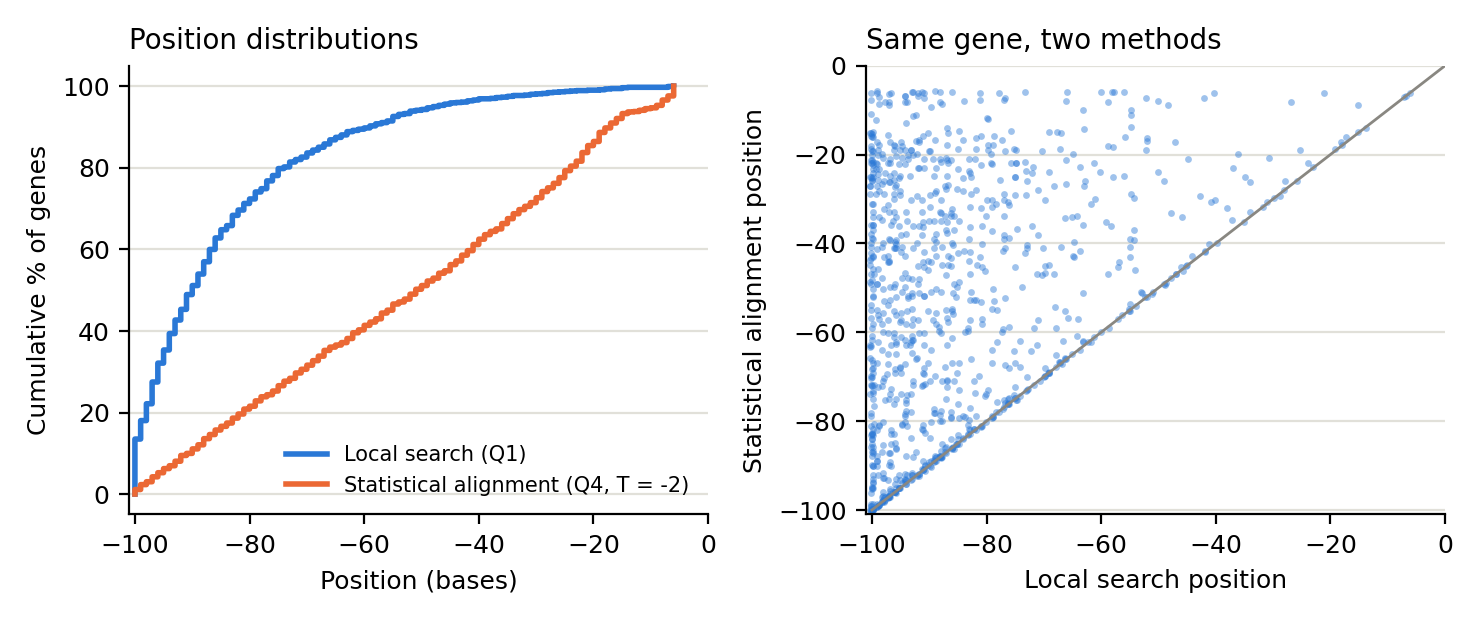
\includegraphics[width=0.9\linewidth]{fig_Q5_positions.png}
\caption{Left: cumulative distribution of the hit position for the two searches. Right: position
found by the statistical alignment against the position found by the local search for the same gene
(points on the diagonal agree).}
\label{fig:q5}
\end{figure}

\paragraph{Percentage of promoters detected.}
Both searches find a potential promoter in front of almost every gene (99.5\%), and with
$T\leq-2$ they find exactly the same 995 genes. This agreement is not a coincidence. The PPM was made
only from intact \seqs{WWWW} hits, so it gives C and G at positions 1--4 a probability of about
$10^{-5}$, and the statistical alignment can only accept windows that the local search would also
accept. It can never be more sensitive than the local search, and with $T=-1$ it is slightly less
sensitive (990 genes).

The more important result is that both percentages are almost the same as the chance level: 97.8\%
of the shuffled sequences contain \seqs{WWWW} and 97.6\% pass the statistical alignment at $T=-2$.
With 54.9\% A/T in the upstream regions, the chance of \seqs{WWWW} at any one position is
$0.549^4=0.091$, so about 8.8 copies are expected in 97 positions, and a random sequence contains at
least one with probability 0.994. In information terms, \seqs{WWWW} carries only 4~bits, but to point
at one site among about 100 positions a pattern needs at least $\log_2 100\approx6.6$~bits~\cite{schneider}.
So the \seqs{WWWW} search mainly measures how A/T-rich a sequence is, not whether it has a promoter.
My data shows this clearly. In 466 of the 1000 genes the upstream region overlaps another gene, and
428 of these come right after another + strand gene, which is how genes are arranged inside an
operon (such genes are transcribed from the operon's promoter and usually have no promoter of their
own). Still, 99.1\% of them came out ``positive''. Real $\sigma^{70}$ promoters are defined by both
boxes and the spacer between them, and natural promoters match only 3--4 of the 6 bases of each
consensus~\cite{harley}, so one short degenerate word cannot identify them.

\paragraph{Position distribution.}
For the same genes, the two searches give very different positions (Figure~\ref{fig:q5}). Only 179
genes (18.0\%) have the same position in both and 241 (24.2\%) are within 2 bases, and the KS test
shows that the two distributions are very different ($D=0.53$, $p<10^{-100}$). The local-search
positions come from the ``first hit'' rule: they pile up at $-100$ and closely follow the shuffled
curve. The statistical alignment instead looks at all ${\sim}12$ candidates in a sequence and picks
the most PPM-like one. Because a detected window must start with \seqs{WWWW} and the local search
returns the first \seqs{WWWW}, the statistical hit is always at the same place or closer to the gene
(median shift 30 bases), and it sits in a longer A/T run (6.4 against 5.5 bases). Most of its
positions (77.6\%) are spread evenly between $-100$ and $-26$, like the shuffled sequences (79.1\%),
but near the gene there is a small difference: more hits between $-25$ and $-14$ (16.1\% against
12.5\% by chance) and between $-8$ and $-6$ (4.7\% against 3.2\%), and fewer between $-13$ and $-9$
(1.6\% against 5.1\%). These regions belong to the translation start region (an A/U-rich stretch
before the SD that helps the ribosome to bind~\cite{boni}, the G-rich SD itself and the A-rich spacer
before the start codon) rather than to a promoter. If the hits were real $-10$ boxes I would expect a
peak at about $-30$ to $-50$, since the TSS is usually 20--40 bases before the start
codon~\cite{mendoza}; neither search shows such a peak.

\paragraph{Which search is better?}
I think the statistical alignment is the better method in principle. It uses every position of the
motif, gives partial credit for near matches according to how often each base was observed, ranks
all the windows of a sequence, and its threshold lets me trade sensitivity against false positives.
In this assignment it could not do better, because its PPM was learned from the output of a
non-specific search and holds only 4.06~bits. The thresholds $-1$ to $-5$ are also too loose for
such a weak matrix: Figure~\ref{fig:thr} shows that the real and shuffled curves only separate
between $T=0$ and about $-0.5$ (for example 11.3\% against 4.8\% at $T=0$, where only the exact
consensus \seqs{ATTTTT} passes, and 94.6\% against 84.8\% at $T=-0.5$). That small gap comes from
the extra A/T tracts found in Q2.

\paragraph{Limitations and improvements.}
If I did this again, I would (i) build the PPM from experimentally confirmed promoters, or at least
from the full \seqs{TATAAT} and \seqs{TTGACA} boxes, instead of from the \seqs{WWWW} hits; (ii) score
windows as log-odds against the genome's base composition so that A/T-rich DNA does not score high by
itself; (iii) search for the $-35$ and $-10$ boxes together with a 15--19 base spacer; (iv) set the
threshold using shuffled or coding sequences so that the false-positive rate is known; and (v) only
use genes that start an operon, because genes inside an operon usually have no promoter.

% =============================================================================
\section{Conclusion}
% =============================================================================
The standard local search found an intact \seqs{WWWW} upstream of 99.5\% of the first 1000
sense-strand genes of \textit{S.~enterica} ASM2286996v1. The hits were mostly far from the genes
(median $-90$) only because the first hit is reported. The A/T runs at the hits were 5.5 bases long
on average and longer than expected by chance. The PPM made from the 6 bases at each hit (consensus
\seqs{ATTTTT}, 4.06~bits) mostly repeated the query, so the statistical alignment detected the same
genes (99.0--99.5\% for $T=-1$ to $-5$) but placed the hit somewhere else (median $-51$; same position
for only 18\% of the genes). Because shuffled sequences give 97.6--97.8\%, I conclude that
\seqs{WWWW} detects A/T-rich DNA rather than real promoters, and that finding promoters reliably needs
a more informative model and a threshold that is set against a background.

% =============================================================================
\begin{thebibliography}{10}
\small
\bibitem{pribnow} D.~Pribnow, ``Nucleotide sequence of an RNA polymerase binding site at an early T7
promoter,'' \textit{PNAS}, vol.~72, pp.~784--788, 1975.
\bibitem{harley} C.~B.~Harley and R.~P.~Reynolds, ``Analysis of \textit{E. coli} promoter
sequences,'' \textit{Nucleic Acids Research}, vol.~15, pp.~2343--2361, 1987.
\bibitem{anastassiou} D.~Anastassiou, ``Genomic signal processing,'' \textit{IEEE Signal Processing
Magazine}, vol.~18, no.~4, pp.~8--20, 2001.
\bibitem{ncbi} NCBI Datasets, genome assembly ASM2286996v1 (GCA\_022869965.1 / GCF\_022869965.1).
\url{https://www.ncbi.nlm.nih.gov/datasets/genome/GCF_022869965.1/}
\bibitem{mendoza} A.~Mendoza-Vargas \textit{et al.}, ``Genome-wide identification of transcription
start sites, promoters and transcription factor binding sites in \textit{E. coli},''
\textit{PLoS ONE}, vol.~4, e7526, 2009.
\bibitem{sw} T.~F.~Smith and M.~S.~Waterman, ``Identification of common molecular subsequences,''
\textit{Journal of Molecular Biology}, vol.~147, pp.~195--197, 1981.
\bibitem{logo} T.~D.~Schneider and R.~M.~Stephens, ``Sequence logos: a new way to display consensus
sequences,'' \textit{Nucleic Acids Research}, vol.~18, pp.~6097--6100, 1990.
\bibitem{stormo} G.~D.~Stormo, ``DNA binding sites: representation and discovery,''
\textit{Bioinformatics}, vol.~16, pp.~16--23, 2000.
\bibitem{sd} J.~Shine and L.~Dalgarno, ``The 3$'$-terminal sequence of \textit{E. coli} 16S
ribosomal RNA: complementarity to nonsense triplets and ribosome binding sites,'' \textit{PNAS},
vol.~71, pp.~1342--1346, 1974.
\bibitem{schneider} T.~D.~Schneider, G.~D.~Stormo, L.~Gold and A.~Ehrenfeucht, ``Information content
of binding sites on nucleotide sequences,'' \textit{Journal of Molecular Biology}, vol.~188,
pp.~415--431, 1986.
\bibitem{boni} I.~V.~Boni, D.~M.~Isaeva, M.~L.~Musychenko and N.~V.~Tzareva, ``Ribosome--messenger
recognition: mRNA target sites for ribosomal protein S1,'' \textit{Nucleic Acids Research}, vol.~19,
pp.~155--162, 1991.
\end{thebibliography}

% =============================================================================
\appendix
\section{Files in the submitted .zip}
{\footnotesize\raggedright
\begin{itemize}[itemsep=0pt,topsep=2pt]
  \item \texttt{data/}: the GenBank genome
        (\texttt{GCA\_022869965.1\_}\allowbreak\texttt{ASM2286996v1\_genomic.fna}) and the protein
        table (\texttt{ncbi\_dataset.tsv}).
  \item \texttt{code/}: \texttt{main.py} runs everything in order and \texttt{assignment1\_notebook.ipynb}
        runs the same functions step by step. The functions are in \texttt{config.py} (settings),
        \texttt{helpers.py}, \texttt{step0\_data.py}, \texttt{step0\_methionine\_check.py},
        \texttt{q1\_local\_search.py}, \texttt{q2\_consecutive\_w.py}, \texttt{q3\_ppm.py},
        \texttt{q4\_statistical\_}\allowbreak\texttt{alignment.py}, \texttt{q5\_comparison.py},
        \texttt{plots.py} and \texttt{summary.py}.
  \item \texttt{results/}: the derived sequences (\texttt{sequences/}, \texttt{.fasta} and
        \texttt{.txt}), the results of every question as \texttt{.csv} tables (\texttt{tables/}), the
        figures, \texttt{summary.json} (all the numbers in this report) and \texttt{run\_log.txt}.
        \texttt{README.txt} explains how to run the code.
\end{itemize}
}

\clearpage
\section{Main parts of my code}
My code is split into one file per step (Appendix~A). These
are the two functions that do the searches.

\begin{lstlisting}[caption={Q1: Smith--Waterman local search with the W letter (from \texttt{q1\_local\_search.py}).}]
def score(query_letter, base):
    """+1 if the base fits the query letter (W fits A and T), otherwise -1."""
    allowed = WEAK if query_letter == "W" else query_letter
    return MATCH if base in allowed else MISMATCH


def local_search(seq, query):
    """Smith-Waterman local alignment of the query against seq.
    Returns (best score, index in seq where the best alignment starts).
    The query is 'intact' when the best score is len(query) * MATCH, which can
    only happen when every query letter is matched with no gap."""
    n, m = len(seq), len(query)
    H = np.zeros((n + 1, m + 1))
    for i in range(1, n + 1):
        for j in range(1, m + 1):
            H[i, j] = max(0,
                          H[i - 1, j - 1] + score(query[j - 1], seq[i - 1]),   # match / mismatch
                          H[i - 1, j] + GAP,                                   # gap in the query
                          H[i, j - 1] + GAP)                                   # gap in the sequence
    best = H.max()
    # np.argmax gives the FIRST cell with the best score, so when there are many
    # equal hits I get the one nearest to the 5' end (the same as max() in MATLAB).
    i, j = np.unravel_index(np.argmax(H), H.shape)
    while i > 0 and j > 0 and H[i, j] > 0:        # trace back to the start of the alignment
        if H[i, j] == H[i - 1, j - 1] + score(query[j - 1], seq[i - 1]):
            i, j = i - 1, j - 1
        elif H[i, j] == H[i - 1, j] + GAP:
            i -= 1
        else:
            j -= 1
    return best, i
\end{lstlisting}

\begin{lstlisting}[caption={Q4: statistical alignment with the PPM (from \texttt{q4\_statistical\_alignment.py}; log\_ppm is the natural log of the PPM).}]
def stat_align(seq, log_ppm):
    """Score every 6-base window of seq: S = ln p(base1, pos1) + ... + ln p(base6, pos6).
    I do it for all windows at once with numpy (the same as two for-loops)."""
    x = to_numbers(seq)
    n_windows = len(x) - WINDOW + 1
    scores = np.zeros(n_windows)
    for j in range(WINDOW):
        scores += log_ppm[x[j:j + n_windows], j]
    return scores


# in run_q4(): best window of every sequence and the detection rule
best_index, best_rel = [], []
for seq in upstream:
    s = stat_align(seq, log_ppm)          # 95 windows, from -100 to -6
    best_index.append(int(np.argmax(s)))   # first best window (5' end side) if there is a tie
    best_rel.append(s.max() - consensus_score)
best_rel = np.array(best_rel)
detected = {t: best_rel >= t for t in THRESHOLDS}
\end{lstlisting}

\end{document}
